%\documentclass[12pt]{article}
%\usepackage{amsmath, amssymb, graphicx}
%\begin{document}
%\title{Chapter 2: Groups \\ Section 6: Cosets}
%\author{Alec Mouri}
%
%\maketitle
%\section*{Exercises}
\begin{itemize}
\item[(1)]
Consider $a \in \mathbb{Z}$, $hn \in n\mathbb{Z}$. Let $b = a + hn$. Using the division algorithm, we can write $a$ as $qn + r$, for $r < n$. So $b = (q + h)n + r$. Let $b_1 = (q_1 + h)n + r_1$, $b_2 = (q_2 + h)n + r_2$. $b_1, b_2$ are in the same coset if and only if $r_1 = r_2$. Since there are $n$ possible values of $r_1$ or $r_2$, then $[\mathbb{Z} : n\mathbb{Z}] = n$.
\item[(2)]
Consider the left cosets $aH$ and $bH$. Suppose for some $c$, $c \in aH$ and $c \in bH$. So $c = ah_1$ and $c = bh_2$, for $h_1, h_2 \in H$. So $ah_1 = bh_2 \rightarrow a = bh_2h_1^{-1}$. So $a \in bH$, ie. $a = bh_b = h_2h_1^{-1}$. So for $x \in aH$, then $x = ah_a = bh_2h_1^{-1}h_a \rightarrow x \in bH$. Thus, $aH \subseteq bH$. Similarly, $bH \subset aH$, so $aH = bH$. Thus, if $aH \neq bH$, then $aH \cap bH = \emptyset$.

Similarly, we can show all distinct right cosets do not overlap.
\item[(3)]
Suppose $G$ has order $p^n$, for $n \geq 1$. If $n = 1$, then $G$ is a cyclic group of order $p$, so for some $a$, $a$ generates $G$, and $a^p = 1$.

Suppose the statement is true for all $n \leq k - 1$. Then if $n = k$, for some $a \in G$, where $a \neq 1$, then $a$ generates some subgroup $H = \left\lbrace 1, a, a^2, ..., a^{x - 1} \right\rbrace$, where $x$ is the order of $a$. From the Counting Theorem, $|H|$ divides $|G|$, ie. $|H|$ is a power of $p$. If $|H| = p^n$, then $|a| = p^n$. So, $|a^{p^{n-1}}| = p$. If $|H| = p^i$, where $i < n$, then by the inductive hypothesis, the statement is true for $H$, and thus also for $G$.
\item[(4)]
Consider
$$H_1 = \begin{bmatrix}
a_1 & b_1 \\
c_1 & d_1
\end{bmatrix}, H_2 = \begin{bmatrix}
a_2 & b_2 \\
c_2 & d_2
\end{bmatrix} \in GL_2(\mathbb{R}), A = \begin{bmatrix}
i & i \\
& 1
\end{bmatrix} \in GL_2(\mathbb{C})$$
Then
$$H_1A = \begin{bmatrix}
a_1 & b_1 \\
c_1 & d_1
\end{bmatrix}\begin{bmatrix}
1 & i \\
& 1
\end{bmatrix} = \begin{bmatrix}
a_1 & b_1 + a_1i \\
c_1 & d_1 + c_1i
\end{bmatrix}$$
And
$$AH_2 = \begin{bmatrix}
1 & i \\
& 1
\end{bmatrix}\begin{bmatrix}
a_2 & b_2 \\
c_2 & d_2
\end{bmatrix} = \begin{bmatrix}
a_2 + c_2i & b_2 + d_2i \\
c_2 & d_2
\end{bmatrix}$$
For $c_2 \neq 0$, then $AH_2 \neq H_1A$. Thus the left and right cosets are different.
\item[(5)]
Since 3 and 5 are prime, then for some $h \neq 1 \in H$ and $k \neq 1 \in K$, then $H = \left\lbrace 1, h, h^2 \right\rbrace$, and $K = \left\lbrace 1, k, k^2, k^3, k^4 \right\rbrace$. Suppose for some $0 \leq i < 5$, $h = k^i$. Then $1 = k^{3i} \rightarrow i = 0 \rightarrow h = 1$, a contradiction The suppose for some $0 \leq j < 5$, then $h^2 = k^j$. Then $1 = k^{3j} \rightarrow j = 0 \rightarrow h^2 = 1$, a contradiction. So, $H \cap K = \left\lbrace 1 \right\rbrace$
\item[(6)]
From (5.13), the left cosets of $\text{ker }\varphi$ are the fibres of $\varphi$. Let $\tau$ map fibres of $\varphi$ onto $\text{im }$. Let $A, B \in \text{im }\varphi$, and $\varphi^{-1}(A), \varphi^{-1}(B)$ be fibres of $\varphi$ on $A$ and $B$ respectively, where $A \neq B$. That is, $\tau(\varphi^{-1}(A)) = A$, and $\tau(\varphi^{-1}(B)) = B$. For $a \in \varphi^{-1}(A), b \in \varphi^{-1}(B)$, then clearly $a \neq b$, and so $\varphi(a) = A, \varphi(b) = B$. So $\tau$ is injective. And since $\varphi$ is surjective onto $\text{im }\varphi$ by definition, then $\tau$ is surjective. Thus, $\tau$ is a bijection. So, $[G: \text{ker }G] = |\text{im }\varphi|$. Thus by the Counting Theorem, $|G| = |\text{ker }\varphi|[G: \text{ker }G] = |\text{ker }\varphi| \cdot |\text{im }\varphi|$.
\item[(7)]
\begin{itemize}
\item[(a)]
Let $a, b \in G$. Then $\varphi(ab) = (ab)^2 = a^2b^2 = \varphi(a)\varphi(b)$. So $\varphi$ is a homomorphism.

Let $H$ be the subgroup generated by $x$. Since $|H|$ divides $|G|$, and $|G|$ is odd, then $|x| = |H| = 2k + 1$ is odd. Let $\tau(x) = x^{k + 1}$. Then $\varphi(\tau(x)) = \tau(\varphi(x)) = x^{2(k+1)} = x$. So, $\varphi$ is a bijection. Thus, $\varphi$ is an automorphism.
\item[(b)]
Claim: Let $G$ be an abelian group. Consider $r$, where $gcd(r, |G|) = 1$, ie. $r$ is relatively prime to $|G|$. Then $\varphi(x) = x^r$ is an automorphism.

Let $a, b \in G$. Then $\varphi(ab) = (ab)^2 = a^2b^2 = \varphi(a)\varphi(b)$. So $\varphi$ is a homomorphism.

Let $H$ be the subgroup generated by $x$. Since $|H|$ divides $|G|$, and $|G|$ is relatively prime with $r$, then $|x| = |H|$ is also relatively prime with $r$. Write $1 = cr + d|H|$ for some $c, d$. Let $\tau(x) = x^{c}$. Then $\varphi(\tau(x)) = \tau(\varphi(x)) = x^{cr} = x^{1 - d|H|} = x$. So, $\varphi$ is a bijection. Thus, $\varphi$ is an automorphism.
\end{itemize}
\item[(8)]
Consider the coset $x+W$, where $Ax = B$. If $y \in x + W$, then $y = x+w$, where $w \in W$. Then $Ay = A(x+w) = Ax + Aw = B$. So, $y$ is a solution to $AX = B$.

Consider $y$ such that $Ay = B$. Then $B = B + 0 = Ay + Aw = A(y + w)$, where $w \in W$. So $y+w \in x+W$.

Therefore, the solutions of $AX = B$ forms a coset.

\item[(9)]
\begin{itemize}
\item[(a)]
Suppose $|G|$ is finite. Then $[G : H]$ is also finite. So there are a finite number of left cosets: $a_1H, a_2H, ..., a_nH$. Let $x \in a_iH \rightarrow x = a_ih$. Then $a_i^{-1}x = h \rightarrow x^{-1}a_i = h^{-1} \rightarrow x^{-1} = h^{-1}a_i \rightarrow x^{-1} \in Ha_i^{-1}$. So there is a 1:1 correspondence between $a_iH$ and $Ha_i^{-1}$. Thus there are $n$ right cosets.
\item[(b)]
Consider the cosets $aH$ and $Ha^{-1}$. Define $\varphi$ as $\varphi(aH) = Ha^{-1}$. Note that if $aH = bH$, then for $h_a, h_b \in H$, $ah_a = bh_b \rightarrow b^{-1}a \in H \rightarrow b^{-1}(a^{-1})^{-1} \in H \rightarrow b^{-1}(a^{-1})^{-1} = h_1h_2 \rightarrow h_1^{-1}b^{-1} = h_2a^{-1} \rightarrow Ha^{-1} = Hb^{-1}$. So $\varphi$ is well defined. Define $\varphi^{-1}(Ha) = a^{-1}H$ Note that $\varphi^{-1}(\varphi(aH)) = aH$, and $\varphi(\varphi^{-1}(Ha)) = Ha$, so there is a bijective correspondence between left and right cosets. Thus the number of left and right cosets are equal.
\end{itemize}
\item[(10)]
\begin{itemize}
\item[(a)]
Consider the two left cosets $aH$ and $bH$. I claim that $aH = Ha$, and $bH = Hb$. Suppose for $ah_1 \in aH$, that $ah_1 \in Hb$. Then for some $h_2$, $ah_1 = h_2b \rightarrow ah_1h_2^{-1} \in b$. So $b \in aH$. But $b \in bH$, and $aH \cap bH = \emptyset$ Thus, $ah_1 \not \in Hb$. Then $ah_1 \in Ha$. Similarly, for $h_1a \in Ha$, then $h_1a \in aH$. Thus, $aH = Ha$. We can similarly show that $bH = Hb$. Therefore, $H$ is normal.
\item[(b)]
Consider the subgroup $H = \left\lbrace 1, xy \right\rbrace$ of $S_3$. Then $H$ has index 3: the left cosets are $H = \left\lbrace 1, xy \right\rbrace, xH = \left\lbrace x, x^2y \right\rbrace, yH = \left\lbrace y, x^2y \right\rbrace$. But the right cosets are $H = \left\lbrace 1, xy \right\rbrace, Hx = \left\lbrace x, y \right\rbrace, Hx^2 = \left\lbrace x^2, x^2y \right\rbrace$. Since the left and right cosets do not correspond, then $H$ is not normal.
\end{itemize}
\item[(11)]
\begin{itemize}
\item[(a)]
If $G$ contains an element $x$ of order 6, then $G$ is	 a cyclic group generated by $x$.

Define $\varphi(x^n) = n \in 6\mathbb{Z}$. Then $\varphi(x) = 1$, so $\varphi$ is a homomorphism. And, let $\tau(n) = x^n$. Then $\varphi(\tau(n)) = 1$, and $\tau(\varphi(x^n)) = x^n$. So, $\varphi$ is a bijection, and is therefore an isomorphism. Thus, $G \simeq 6Z$
\item[(b)]
Suppose $G$ is abelian, ie. $xy = yx$. Let $x$ be of order 3. $y$ is of order $2$ or $3$. If $y$ is of order 3, then $J = \left\lbrace 1, y, y^2 \right\rbrace$ is a subgroup of $G$. Note that $y \in H$ (otherwise $H + J = \left\lbrace 1, x, x^2, y, y^2 \right\rbrace$, so $1 \neq a \not \in H + J$ has order 1, a contradiction), so $H = J$. Thus there exists some $y$ such that $y$ has order 2. Then $6$ is the order of $xy$, a contradiction. So $G$ is not abelian. 

Let $a$ have order 3 and $b$ have order 2. Then $\varphi(a^ib^j) = x^ib^j$. Thus is clearly an isomophism. Thus $G \simeq S_3$.
\item[(c)]
Suppose all elements of $G$ have order 1 or 2. Let $x, y \in G$. Then $(xy)^2 = y^2 = 1$. Then $xy = yx$. So $G$ is abelian. But, for distinct $x, y, z$, then $1, x, y, z, xy, yz, xz$ are all distinct. Thus $G$ does not exist.
\end{itemize}
\item[(12)]
Let 
$$A = \begin{bmatrix}
a_1 & a_2 \\
0 & 1
\end{bmatrix}$$
Then
$$AH = \begin{bmatrix}
a_1 & a_2 \\
0 & 1
\end{bmatrix}\begin{bmatrix}
x & 0 \\
0 & 1
\end{bmatrix} = \begin{bmatrix}
xa_1 & a_2 \\
0 & 1
\end{bmatrix}$$
And
$$HA = \begin{bmatrix}
x & 0 \\
0 & 1
\end{bmatrix}\begin{bmatrix}
a_1 & a_2 \\
0 & 1
\end{bmatrix} = \begin{bmatrix}
xa_1 & xa_2 \\
0 & 1
\end{bmatrix}$$
Left cosets: \\
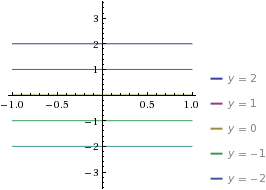
\includegraphics[scale=2.0]{fig/C2_S6_12-1} \\
Right cosets: \\
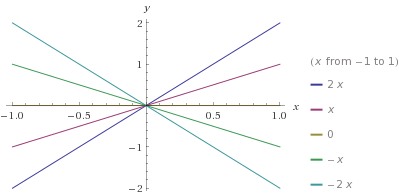
\includegraphics[scale=1.5]{fig/C2_S6_12-2}
\end{itemize}
%\end{document}